\documentclass[14pt, a4paper]{extarticle}
\usepackage{mospolytech_coursework} 

\usepackage{ragged2e}
\usepackage{longtable}
\usepackage{tabularx}
\usepackage{calc}

\usepackage{caption}
\captionsetup[figure]{skip=12pt}


\newcolumntype{P}[1]{>{\RaggedRight\arraybackslash}p{#1 - 2\tabcolsep - 2\arrayrulewidth}}
\newcolumntype{C}[1]{>{\centering\arraybackslash}p{#1 - 2\tabcolsep - 2\arrayrulewidth}}

\newcommand{\subject}{Разработка веб-приложений}
\newcommand{\theme}{Разработка веб-приложения „Книга снов“ с личными кабинетами пользователей для ведения дневника сновидений и статистического анализа}
\newcommand{\student}{Кленечева Анастасия Владимировна}
\newcommand{\group}{241-327}
\newcommand{\teacher}{Кружалов Алексей Сергеевич}


\renewcommand{\thesection}{\arabic{section}}
\renewcommand{\thesubsection}{\arabic{section}.\arabic{subsection}}

% Настройка формата подразделов
\renewcommand{\thesubsection}{\arabic{section}.\arabic{subsection}}

% Отключаем нумерацию на первых страницах
\pagestyle{empty}

\begin{document}

% ==================== ТИТУЛЬНЫЙ ЛИСТ ====================

\begin{center}
    {\small Министерство науки и высшего образования Российской Федерации}
    
    \resizebox{\textwidth}{!}{\fontsize{8pt}{10pt}\selectfont Федеральное 
    государственное автономное образовательное учреждение высшего образования} 
    
    {\small \textbf{«МОСКОВСКИЙ ПОЛИТЕХНИЧЕСКИЙ УНИВЕРСИТЕТ»}} \\
    {\small \textbf{(МОСКОВСКИЙ ПОЛИТЕХ)}}

    \vspace{4cm}

    {\Large \textbf{КУРСОВОЙ ПРОЕКТ}} \\[1cm]
    {\large по курсу \\ «\subject»}

    \vspace{1.5cm}

    \textbf{ТЕМА} \\[0.3cm]
    {\large «\theme»}

    \vspace{3cm}

    \hfill
    \begin{tabular}{p{3cm} l}
        \textbf{Выполнил:} & \student \\
        \textbf{Группа:}   & \group \\
        \\
        \textbf{Проверил:}  & \teacher
    \end{tabular}

    \vfill

    Москва, 2026
\end{center}

\newpage

% ==================== ЗАДАНИЕ ====================

\begin{center}
    {\small Министерство науки и высшего образования Российской Федерации}

    \resizebox{\textwidth}{!}{\fontsize{8pt}{10pt}\selectfont Федеральное 
    государственное автономное образовательное учреждение высшего образования}

    {\small \textbf{«МОСКОВСКИЙ ПОЛИТЕХНИЧЕСКИЙ УНИВЕРСИТЕТ»}} \\
    {\small \textbf{(МОСКОВСКИЙ ПОЛИТЕХ)}}
\end{center}

\noindent
\hfill
\begin{tabularx}{\textwidth}{@{} p{0.53\textwidth} p{0.43\textwidth} @{}}
     &
    \raggedright
    УТВЕРЖДАЮ                          \\
    заведующая кафедрой                \\
    «Инфокогнитивные технологии»       \\[0.3cm]

    \rule{3cm}{0.4pt} / Е.~А.~Пухова / \\[0.1cm]

    «\rule{0.8cm}{0.4pt}» \rule{3cm}{0.4pt} 2026~г.
\end{tabularx}

\vspace{1cm}

\begin{center}
    {\large \textbf{ЗАДАНИЕ}}
    
    \textbf{на выполнение курсовой работы (проекта)}
    
    Кленечевой Анастасии Владимировне,
\end{center}

\noindent обучающейся группы 241-327,\\
 направления подготовки 09.03.01 «Информатика и вычислительная техника»\\
 по дисциплине «Разработка веб-приложений»\\
 на тему «\theme».


\noindent {1. Исходные данные к работе (проекту):} информационные ресурсы в сети интернет, научные публикации в открытой печати.

\noindent {2. Содержание задания по курсовой работе (проекту) -- перечень вопросов, подлежащих разработке:}

{
\renewcommand{\arraystretch}{1.2}
\footnotesize
\begin{longtable}{|P{0.5\textwidth}|C{0.11\textwidth}|C{0.15\textwidth}|C{0.24\textwidth}|}
    \hline
    \textbf{Разрабатываемый вопрос} & \textbf{Объем, \%} & \textbf{Срок} & \textbf{Примечание} \\
    \hline
    \endhead
    \hline
    \endfoot

\multicolumn{4}{|P{\textwidth}|}{\textbf{Раздел 1. Анализ предметной области}} \\ \hline
Задача 1.1. Обзор существующих решений & 10 & 22.03.2026 & Анализ аналогов \\ \hline
Задача 1.2. Анализ инструментов разработки & 7 & 26.03.2026 & Выбор стека \\ \hline
Задача 1.3. Формулировка цели и задач & 8 & 30.03.2026 & Постановка ТЗ \\ \hline

\multicolumn{4}{|P{\textwidth}|}{\textbf{Раздел 2. Проектирование}} \\ \hline
Задача 2.1. Анализ целевой аудитории & 5 & 02.04.2026 & Портрет пользователя \\ \hline
Задача 2.2. Описание функциональности & 7 & 06.04.2026 &  \\ \hline
Задача 2.3. Проектирование модели данных & 8 & 10.04.2026 & ER-диаграмма \\ \hline
Задача 2.4. Разработка макетов страниц & 5 & 14.04.2026 &  \\ \hline

\multicolumn{4}{|P{\textwidth}|}{\textbf{Раздел 3. Разработка}} \\ \hline
Задача 3.1. Модели БД & 5 & 17.04.2026 &  \\ \hline
Задача 3.2. Аутентификация и личные кабинеты & 5 & 21.04.2026 & \\ \hline
Задача 3.3. CRUD для снов & 6 & 25.04.2026 & Базовый функционал \\ \hline
Задача 3.4. Загрузка файлов & 6 & 29.04.2026 & \\ \hline
Задача 3.5. Анализ текста сна & 6 & 04.05.2026 & Поиск символов \\ \hline
Задача 3.6. Агрегация данных и статистика & 7 & 09.05.2026 & Аналитика \\ \hline
Задача 3.7. Экспорт в CSV & 4 & 19.05.2026 & Отчёт \\ \hline
Задача 3.8. Панель администратора & 6 & 24.05.2026 & Модерация \\ \hline

\multicolumn{4}{|P{\textwidth}|}{\textbf{Раздел 4. Оформление итогов}} \\ \hline
Задача 4.1. Git-репозиторий & 3 & 22.03.2026 & \\ \hline
Задача 4.2. Деплой на хостинг & 4 & 26.05.2026 & Публикация \\ \hline
Задача 4.3. Оформление отчёта & 3 & 26.05.2026 & Пояснительная записка \\ \hline
\end{longtable}
}

\noindent Руководитель курсовой работы (проекта): \\ 
\noindent старший преподаватель кафедры «Инфокогнитивные технологии»

{
\renewcommand{\arraystretch}{2}
\noindent
\begin{tabularx}{\textwidth}{@{} P{0.45\textwidth} P{0.3\textwidth} P{0.25\textwidth} @{}}
    «\rule{0.8cm}{0.4pt}» \quad \rule{2cm}{0.4pt} \quad 2026~г. &
    \centering \rule{3.5cm}{0.4pt} \par \footnotesize (подпись) &
    \hfill А.~С.~Кружалов \\
\end{tabularx}

\noindent
\begin{tabularx}{\textwidth}{@{} P{0.45\textwidth} P{0.55\textwidth} @{}}
    Дата выдачи задания & \hfill «30» \quad марта \quad 2026~г. \\
    Дата сдачи выполненной работы & \hfill «13» \quad июня \quad 2026~г. \\
\end{tabularx}
}

\noindent Задание приняла к исполнению

{
\renewcommand{\arraystretch}{1.5}
\noindent
\begin{tabularx}{\textwidth}{@{} P{0.45\textwidth} P{0.3\textwidth} P{0.25\textwidth} @{}}
    «30» \quad марта \quad 2026~г. &
    
\includegraphics[height=1.6cm]{img/signature.jpg} \par \footnotesize (подпись) &
    \hfill А.~В.~Кленечева \\
\end{tabularx}
}

% ==================== ВКЛЮЧАЕМ НУМЕРАЦИЮ С 5 СТРАНИцы ====================

\newpage
\setcounter{page}{5}
\pagestyle{plain}

% ==================== СОДЕРЖАНИЕ (АВТОМАТИЧЕСКОЕ) ====================


\tableofcontents

\newpage

% ==================== ВВЕДЕНИЕ ====================

\section*{ВВЕДЕНИЕ}
\addcontentsline{toc}{section}{ВВЕДЕНИЕ}

\textbf{Проблема исследования.} Сновидения являются важным источником информации 
о психоэмоциональном состоянии человека и его подсознательных процессах. 
Ведение дневника сновидений традиционно используется в психотерапии и 
самоанализе. Однако существующие способы фиксации снов — бумажные дневники, 
текстовые файлы или приложения-заметки — не позволяют автоматически 
анализировать содержание снов, выявлять повторяющиеся символы или 
визуализировать статистику. Таким образом, проблема заключается в отсутствии 
доступного специализированного инструмента, сочетающего личный дневник 
сновидений с аналитикой данных.

\textbf{Актуальность темы.} В последние годы наблюдается рост интереса к 
велнес-технологиям, направленным на поддержание психического здоровья и 
саморазвитие. Возможность вести структурированный дневник снов и получать 
статистический анализ своих записей повышает вовлечённость пользователя и 
способствует более глубокому осмыслению сновидений. Разработка веб-приложения, 
предоставляющего каждому пользователю личную «Книгу снов» с возможностью 
анализа и визуализации данных, является актуальной задачей на стыке психологии, велнес-технологий и веб-разработки.

\textbf{Степень разработанности проблемы.} В настоящее время существуют 
отдельные решения для ведения дневников сновидений: мобильные приложения 
«Elsewhere», «Dreamovy», «Awoken». Анализ аналогов показывает, что большинство 
из них либо перегружены платными функциями, либо примитивны и не предоставляют 
возможностей для анализа данных. Приложения, поддерживающие статистический 
анализ, встречаются редко. Таким образом, создание веб-приложения с концепцией 
«Книги снов», объединяющей дневник и аналитику, является практической задачей.

\textbf{Объект исследования} — процессы ведения, систематизации и анализа 
дневников сновидений с использованием веб-технологий и генеративных нейросетей.

\textbf{Предмет исследования} — программные средства для создания 
веб-приложения «Книга снов», обеспечивающего личные кабинеты пользователей, 
CRUD-операции с записями, статистическую обработку текстов снов и экспорт данных.

\textbf{Целью данной работы} является проектирование и реализация 
клиент-серверного веб-приложения «Книга снов» для ведения дневника сновидений 
с личными кабинетами и статистическим анализом.

\textbf{Задачи исследования:}
\begin{itemize}
    \item провести анализ существующих решений и обосновать выбор технологий;
    \item спроектировать архитектуру приложения и модель данных;
    \item разработать систему аутентификации и разграничения прав доступа 
    по ролям;
    \item реализовать CRUD-интерфейс для управления записями снов;
    \item разработать модуль агрегации данных для статистического анализа;
    \item реализовать экспорт данных в CSV;
    \item выполнить оформление итогов работы.
\end{itemize}

\textbf{Практическая значимость работы.} Разработанное веб-приложение может 
быть использовано для ведения личного дневника сновидений, а также психологами 
для сбора и анализа данных. Анализ символов и эмоционального фона позволяет 
пользователю лучше понимать свои подсознательные процессы.


\newpage

% ==================== Глава 1 ====================

\section{Анализ предметной области}

\subsection{Обзор существующих решений}

Для определения места разрабатываемого приложения на рынке и выявления
недостатков аналогов проведём анализ существующих решений для ведения
дневников сновидений. На сегодняшний день наиболее популярными являются
мобильные приложения, так как они позволяют делать запись сразу после
пробуждения. Рассмотрим три характерных представителя.

\textbf{Dreamovy (Android/iPhone).} Приложение с акцентом на категоризацию
снов по темам (страхи, мечты, повторяющиеся сны). Позволяет вести
дневник, ставить оценки эмоциональному фону, имеет базовую статистику
(календарь снов). Бесплатная версия ограничена количеством записей,
реклама. Плюсы: удобная категоризация. Минусы: нет анализа символов,
платный доступ к расширенной статистике.

\textbf{Awoken (Android).} Приложение для практикующих осознанные
сновидения. Содержит напоминания для выполнения «проверок реальности»,
звуковые сигналы, а также дневник с тегами. Полностью бесплатное.
Плюсы: удобно для пользователей, открытый исходный код. Минусы: очень
простая аналитика — только текстовый поиск по дневнику, нет графиков,
нет визуализации символов.

\textbf{Lucid Dreamer (iPhone).} Платное приложение с акцентом на
аудиодневник (запись голосом сразу после пробуждения). Поддерживает
облачное резервное копирование. Плюсы: удобный голосовой ввод, красивое
оформление. Минусы: отсутствие статистического анализа, нет экспорта
данных, подписка стоит около 3000 руб./год.

На основе анализа выделим ключевые критерии, важные для пользователей:
поддержка аналитики символов, визуализация данных, наличие тегов/категорий,
экспорт данных, стоимость, веб-доступ. Сравнение представлено в таблице
\ref{tab:competitors_analysis}.

\begin{table}[ht!]
	\centering
	\caption{Сравнительный анализ приложений для ведения дневников сновидений}
	\label{tab:competitors_analysis}
	\footnotesize
	\begin{tabular}{|p{8.5cm}|c|c|c|}
		\hline
		\textbf{Критерий} &
		\textbf{Dreamovy} &
		\textbf{Awoken} &
		\textbf{Lucid Dreamer} \\
		\hline
		Анализ символов/паттернов         & – & – & –  \\
		\hline
		Визуализация статистики (графики)  & \(\pm\) (базовая) & – & – \\
		\hline
		Наличие тегов / категорий          & + & + & – \\
		\hline
		Экспорт данных (PDF/CSV)           & – & – & – \\
		\hline
		Бесплатная версия (базовый функционал) & \(\pm\) (ограничена) & + & – \\
		\hline
		Голосовой ввод / аудиодневник      & – & – & + \\
		\hline
		Веб-доступ (с любого устройства)   & – & – & – \\
		\hline
        Наличие ИИ (генерация иллюстраций / анализ) & – & – & – \\
		\hline
	\end{tabular}
\end{table}

Анализ таблицы показывает, что ни одно из рассмотренных приложений не
предоставляет полноценного статистического анализа текста снов
(частотность символов, эмоциональные тренды), не поддерживает экспорт
данных в PDF и не имеет веб-интерфейса. Приложение «Книга снов» призвано
заполнить эти пробелы, сочетая личный дневник с аналитикой и доступом
через браузер.

\subsection{Анализ инструментов разработки}

Для реализации веб-приложения «Книга снов» необходимо выбрать
оптимальный стек технологий, обеспечивающий производительность,
удобство разработки и достаточный уровень безопасности. Проведём
сравнительный анализ наиболее популярных инструментов для создания
веб-приложений аналогичного класса.

\textbf{Сравнение технологий бэкенда.} Бэкенд-часть отвечает за обработку запросов, взаимодействие с базой
данных, аутентификацию пользователей и бизнес-логику. Рассмотрим три
распространённых подхода: классический синхронный (PHP), асинхронный
на Python (Flask/Django) и корпоративный на Java (Spring). Сравнение
представлено в таблице~\ref{tab:backend_comparison}.

\begin{table}[ht!]
	\centering
	\caption{Сравнительный анализ технологий бэкенда}
	\label{tab:backend_comparison}
	\footnotesize
	\begin{tabular}{|p{7.8cm}|c|c|c|}
		\hline
		\textbf{Критерий} & \textbf{PHP (Laravel)} & \textbf{Python (Flask/Django)} & \textbf{Java (Spring)} \\
		\hline
		Порог входа            & низкий         & низкий          & высокий \\
		\hline
		Скорость разработки    & высокая        & высокая         & средняя \\
		\hline
		Производительность     & средняя        & средняя         & высокая \\
		\hline
		Экосистема библиотек   & широкая        & очень широкая   & широкая \\
		\hline
	\end{tabular}
\end{table}

Анализ таблицы показывает, что Java (Spring) избыточна для небольшого
веб-приложения; PHP (Laravel) также применим, однако экосистема
Python предоставляет более удобные инструменты для анализа текстов
(библиотеки NLTK, pymorphy2) и быстрого прототипирования.

\textbf{Сравнение технологий фронтенда.} Фронтенд-часть определяет пользовательский интерфейс и взаимодействие
с сервером. На рынке доминируют три подхода: классический
(HTML/CSS/JS без фреймворков), React и Vue.js. Сравнение приведено
в таблице~\ref{tab:frontend_comparison}.

\begin{table}[ht!]
	\centering
	\caption{Сравнительный анализ технологий фронтенда}
	\label{tab:frontend_comparison}
	\footnotesize
	\begin{tabular}{|p{8.8cm}|c|c|c|}
		\hline
		\textbf{Критерий} & \textbf{Чистый JS} & \textbf{React} & \textbf{Vue.js} \\
		\hline
		Порог входа            & низкий      & средний    & низкий \\
		\hline
		Скорость разработки    & низкая      & высокая    & высокая \\
		\hline
		Интерактивность UI     & ручная реализация & высокая & высокая \\
		\hline
		Экосистема             & базовая     & огромная   & растущая \\
		\hline
		Подходит для анализа данных & – & + & + \\
		\hline
	\end{tabular}
\end{table}

\newpage
Анализ показывает, что использование чистого JavaScript без фреймворков
приводит к значительному росту объёма кода при реализации динамического
интерфейса (графики, формы, асинхронные запросы). React и Vue.js
одинаково хорошо подходят для визуализации статистики, однако React
обладает более широкой экосистемой.

\textbf{Выбор стека технологий для проекта.} На основе проведённого сравнительного анализа для реализации
веб-приложения «Книга снов» выбран следующий стек технологий:

\begin{itemize}
	\item \textbf{Бэкенд:} язык Python, микрофреймворк Flask.
	      Python обеспечивает простоту написания серверной логики,
	      широкий выбор библиотек для анализа текстов и аутентификации.
	      Flask даёт гибкость, необходимую для небольшого приложения
	      с чётко определённой функциональностью.
	\item \textbf{База данных:} SQLite.
	      Простейшая СУБД, отлично подходящая для хранения записей
	      снов, пользовательских данных и статистики.
	\item \textbf{Фронтенд:} HTML5, CSS3, Bootstrap 5, чистый JavaScript.
	      Выбран классический подход без тяжёлых фреймворков, так как
	      приложение не требует сложной клиентской маршрутизации,
	      а Bootstrap 5 обеспечивает адаптивный интерфейс «из коробки».
	\item \textbf{Дополнительные библиотеки:} Flask-SQLAlchemy (ORM),
	      Flask-Login (аутентификация), Fetch API (асинхронные запросы).
\end{itemize}

Таким образом, выбранный стек технологий полностью покрывает
функциональные требования к приложению «Книга снов» и соответствует
современным практикам веб-разработки.

\newpage

\subsection{Формулировка цели и задач}

На основе проведенного анализа инструментов (см. подраздел 1.2) и выявленных пробелов в существующих продуктах, была сформулирована цель исследования.

\textbf{Цель работы} — создание веб-приложения «Книга снов», обеспечивающего ведение личного дневника сновидений с возможностью статистического анализа записей.

Для достижения поставленной цели необходимо решить следующие \textbf{задачи}:
\begin{enumerate}
	\item Провести сравнительный анализ существующих решений для ведения дневников сновидений и обосновать выбор технологического стека;
	\item Разработать архитектуру клиент-серверного приложения и спроектировать структуру базы данных для хранения записей снов и пользовательских данных;
	\item Реализовать программные модули для аутентификации пользователей и разграничения прав доступа по ролям;
	\item Реализовать CRUD-интерфейс для управления записями снов и агрегации статистических данных;
	\item Разработать модуль экспорта дневника в CSV и провести тестирование разработанной системы.
\end{enumerate}

\newpage

% ==================== Глава 2 ====================

\section{Проектирование веб-приложения}

\subsection{Анализ целевой аудитории}

Для определения функциональных требований к веб-приложению «Книга снов» 
был проведён анализ целевой аудитории. В отличие от корпоративных систем, 
разрабатываемое приложение ориентировано на частных пользователей с 
различными внутренними мотивациями. На основе исследования существующих 
решений выделены три ключевых сегмента пользователей.

\textbf{Первый сегмент — психологически ориентированные пользователи.} 
К этой группе относятся люди, которые ведут дневник сновидений для 
самоанализа, отслеживания эмоционального состояния или в рамках 
психотерапии. Для них ценность приложения заключается в способности 
автоматически выявлять повторяющиеся символы и паттерны, а также 
визуализировать динамику эмоционального фона.

\textbf{Второй сегмент — творческие люди} (писатели, художники, 
сценаристы). Они используют сны как источник образов и вдохновения. 
Для этой аудитории важна эстетическая составляющая: оформление в виде 
«книги», возможность генерации иллюстраций к снам с помощью ИИ, а также 
удобная навигация по архиву записей.

\textbf{Третий сегмент — практикующие осознанные сновидения.} 
Это пользователи, которые целенаправленно работают над развитием навыка 
осознания себя во сне. Их ключевые потребности — отслеживание частоты 
снов, фиксация прогресса, календарь с визуальной индикацией.

Для более детального понимания потребностей каждого сегмента 
был применён метод персонажей (Personas). 

\textit{Персонаж 1: Анна, 32 года, психолог.} Анна ведёт дневник 
сновидений уже два года, используя обычные заметки в телефоне. Она хочет 
отслеживать, какие символы (вода, огонь, падение, полёт) повторяются в её 
снах в периоды стресса. Главная «боль»: существующие приложения не дают 
аналитики, приходится просматривать записи вручную. Приоритетные функции: 
график эмоций, облако тегов, экспорт статистики в CSV.

\textit{Персонаж 2: Дмитрий, 25 лет, художник.} Дмитрий часто видит 
яркие сны и хочет сохранять их не только текстом, но 
и визуально. Ему интересна функция автоматической генерации иллюстрации 
к сну через нейросеть. Также он хочет красиво оформить архив своих снов. 
Приоритетные функции: генерация картинки по тексту сна, экспорт в CSV как 
«книга снов».

\textit{Персонаж 3: Елена, 29 лет, практик осознанных сновидений.} 
Елена уже три года тренирует осознанность во сне и ведёт подробный 
дневник. Ей важно отслеживать частоту снов по дням, отмечать, в какие 
ночи были осознанные сновидения. Елена не хочет тратить время на ручное 
форматирование записей, ей нужен быстрый ввод и наглядный календарь. 
Приоритетные функции: календарь снов, статистика частоты, быстрая 
регистрация сна.

Помимо обычных пользователей, в системе предусмотрена роль 
\textbf{администратора}. Администратор выполняет обслуживающие функции: 
управление справочником символов (добавление, редактирование, удаление), 
блокировка пользователей, просмотр общей статистики.

Проведённый анализ целевой аудитории позволяет сформулировать 
следующие выводы: приложение должно поддерживать три основные группы 
пользователей, каждая из которых имеет свои приоритетные функции; 
интерфейс не должен быть перегружен, но обязан предоставлять доступ ко 
всем ключевым функциям; роль администратора должна быть выделена отдельно 
с расширенными правами.

\subsection{Описание функциональности приложения}

Функциональные возможности системы определяются через взаимодействие пользователя с системой. На основе анализа целевой аудитории (см. раздел 2.1) были сформулированы следующие пользовательские истории (User Stories).

\textbf{Пользовательская история для психологически ориентированного пользователя:} «Как психологически ориентированный пользователь, я хочу автоматически получать статистику по повторяющимся символам в моих снах и график эмоционального фона, чтобы отслеживать своё психоэмоциональное состояние в динамике».

\textit{Критерии приёмки:}
\begin{itemize}
    \item система выделяет из текста сна ключевые символы;
    \item доступен график эмоционального фона по датам;
    \item облако тегов визуализирует самые частые символы.
\end{itemize}

\textbf{Пользовательская история для творческого пользователя:} «Как творческий пользователь, я хочу прикреплять к снам изображения и экспортировать дневник в PDF, чтобы сохранять визуальные образы снов».

\textit{Критерии приёмки:}
\begin{itemize}
    \item загрузка изображений к любому сну;
    \item галерея снов с миниатюрами;
    \item экспорт всей книги снов в CSV с текстом и картинками.
\end{itemize}

\textbf{Пользовательская история для практикующего осознанные сновидения:} «Как практикующий осознанные сновидения, я хочу быстро вносить записи и видеть календарь с отмеченными днями снов, чтобы отслеживать прогресс».

\textit{Критерии приёмки:}
\begin{itemize}
    \item минимальная форма создания сна;
    \item календарь с цветовой индикацией дней со снами;
    \item переход по клику на день к записи сна.
\end{itemize}

На рисунке~\ref{fig:use_case} представлена диаграмма вариантов использования (Use Case), обобщающая все сценарии.

\begin{figure}[ht!]
    \centering
    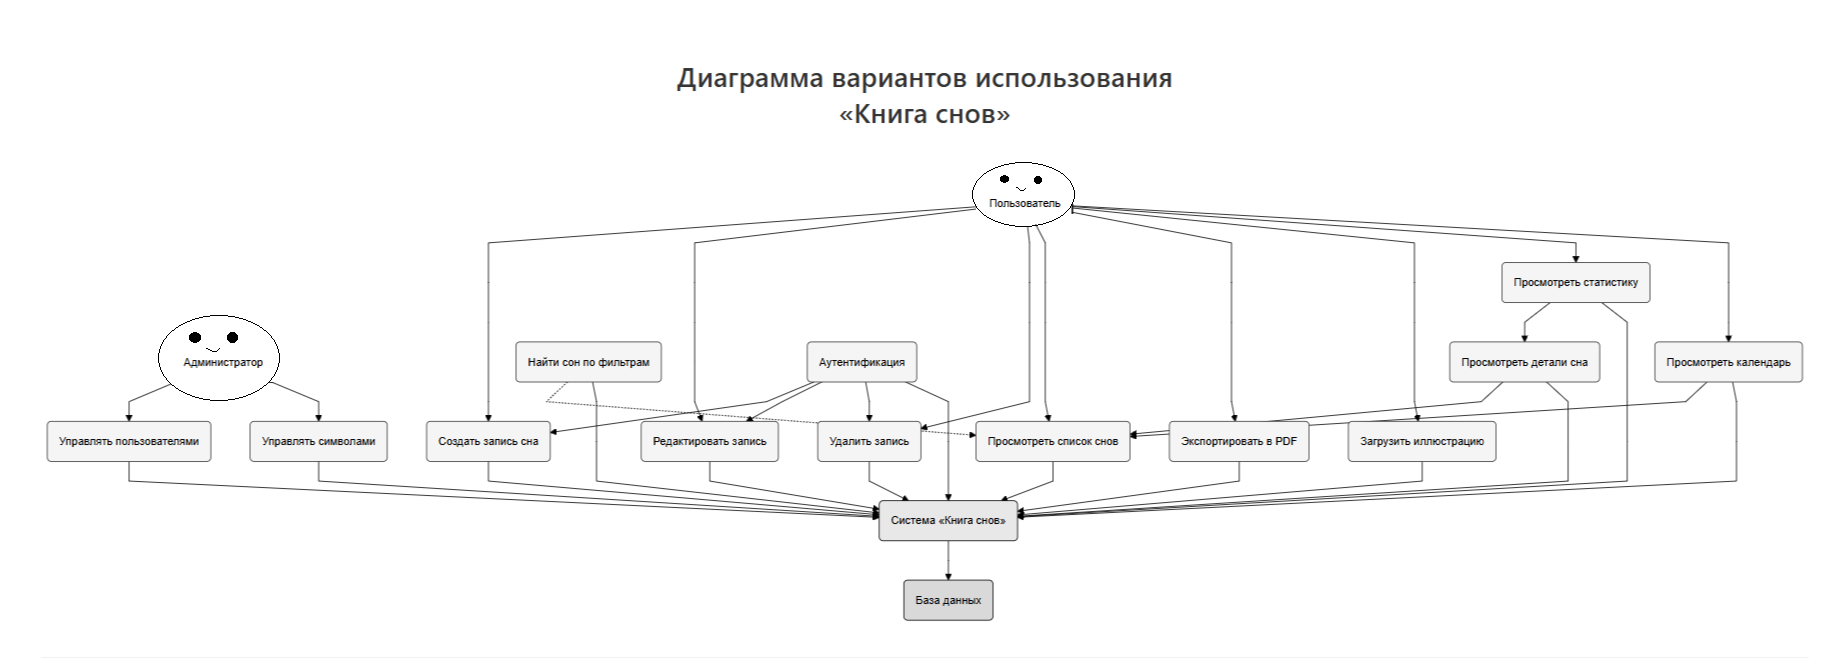
\includegraphics[width=0.95\textwidth]{img/use_case.png}
    \caption{Диаграмма вариантов использования системы «Книга снов»}
    \label{fig:use_case}
\end{figure}

\newpage
\subsection{Проектирование модели данных}

При выборе архитектуры базы данных был проведен сравнительный анализ эффективности различных решений, опирающийся на данные о производительности современных СУБД.

В таблице~\ref{tab:db_comparison} представлено сравнение наиболее популярных реляционных СУБД.

\begin{table}[ht!]
    \centering
    \caption{Сравнительный анализ СУБД для задач «Книги снов»}
    \label{tab:db_comparison}
    \footnotesize
    \begin{tabular}{|p{4.5cm}|c|c|c|}
        \hline
        \textbf{Критерий} & \textbf{PostgreSQL} & \textbf{MySQL} & \textbf{SQLite} \\
        \hline
        Полнотекстовый поиск по тексту & ++ (встроенный, мощный) & + (есть, но слабее) & – (нет) \\
        \hline
        Хранение и поиск по JSON & ++ (отличная поддержка) & + (базовая) & – (нет) \\
        \hline
        Поддержка массивов (для хранения символов) & ++ (есть тип array) & – (нет) & – (нет) \\
        \hline
        Работа с большим количеством записей (1000+) & ++ & ++ & – (тормозит) \\
        \hline
        Поддержка внешних ключей и ссылочной целостности & ++ & ++ (только InnoDB) & + \\
        \hline
        Простота развёртывания для курсовой & средняя & средняя & высокая \\
        \hline
        Бесплатная лицензия & Да & Да & Да \\
        \hline
    \end{tabular}
\end{table}

На основе проведённого анализа для реализации веб-приложения «Книга снов» выбрана СУБД \textbf{SQLite}. Данный выбор обусловлен следующими преимуществами:


\textbf{Структура базы данных.} Спроектированная база данных состоит из девяти таблиц, обеспечивающих хранение пользовательской информации, записей снов, символов для анализа, а также данных для статистики и ИИ-генерации изображений.

\newpage
\textbf{Основные таблицы:}
\begin{itemize}
    \item \texttt{users} — хранит учётные записи пользователей (логин, хеш пароля, роль, аватар, дата регистрации);
    \item \texttt{dreams} — содержит записи снов (заголовок, текст, дата сна, оценка настроения, внешний ключ на пользователя);
    \item \texttt{symbols} — справочник символов для анализа текстов (вода, огонь, полёт и т.д.);
    \item \texttt{dream\_symbols} — связующая таблица для реализации отношения «многие ко многим» между снами и символами.
    \item \texttt{user\_images} — хранит изображения, загруженные пользователем самостоятельно (не через ИИ-генерацию).
\end{itemize}

\textbf{Таблицы для аналитики и кэширования:}
\begin{itemize}
    \item \texttt{statistics} — хранит кэшированную статистику в формате JSON для быстрого отображения;
    \item \texttt{emotion\_stats} — содержит сводки по эмоциональному фону (дневные, недельные, месячные);
    \item \texttt{symbol\_stats} — хранит частоту встречаемости символов по периодам.
\end{itemize}

\textbf{Таблицы для ИИ-генерации:}
\begin{itemize}
    \item \texttt{generation\_requests} — фиксирует запросы к ИИ (промпт, статус выполнения, временная метка);
    \item \texttt{generated\_images} — хранит URL сгенерированных изображений и связь с соответствующим сном и запросом.
\end{itemize}

\newpage
ER-диаграмма, визуализирующая описанные сущности и связи, представлена на рисунке~\ref{fig:er_diagram}.

\begin{figure}[ht!]
    \centering
    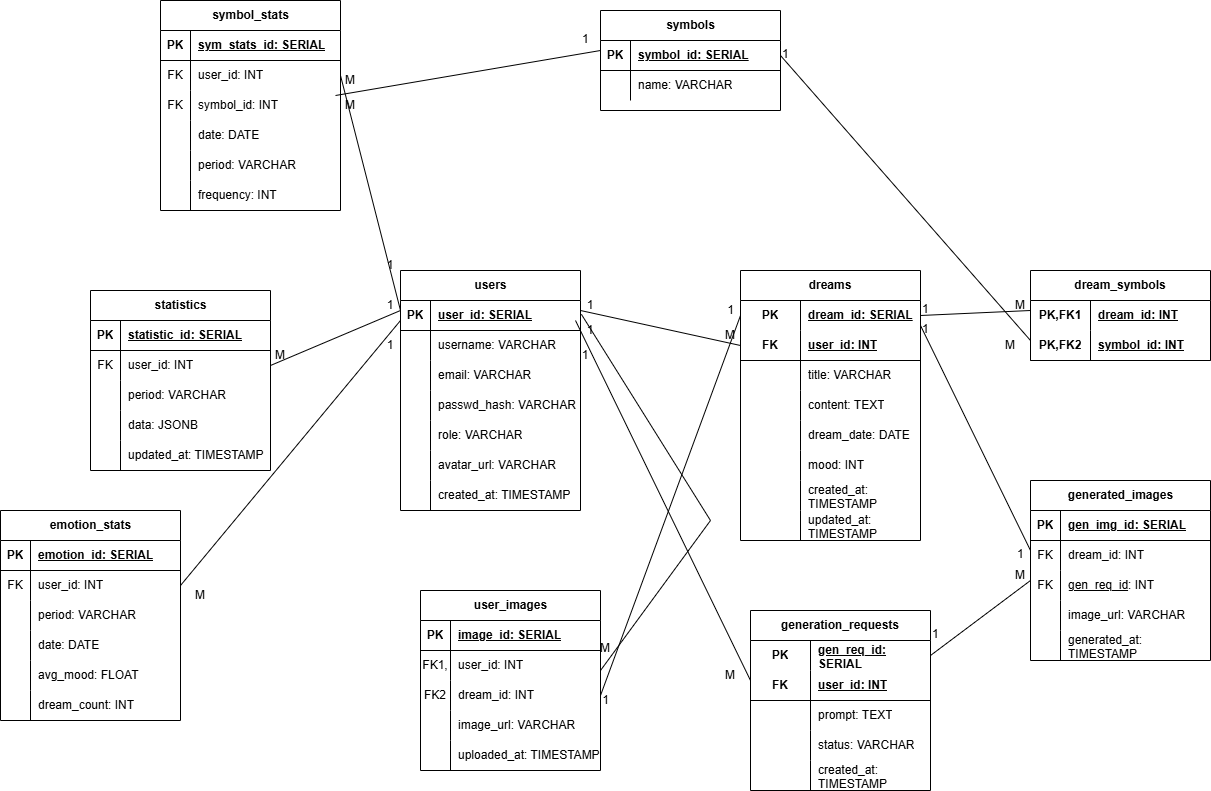
\includegraphics[width=0.9\textwidth]{img/er.png}
    \caption{ER-диаграмма базы данных «Книга снов»}
    \label{fig:er_diagram}
\end{figure}


\subsection{Разработка макетов страниц}

На основе спроектированной функциональности и модели данных были разработаны макеты основных страниц веб-приложения «Книга снов». Макеты выполнены в стиле вайрфреймов (wireframes), демонстрирующих расположение ключевых элементов интерфейса.

\textbf{Макет страницы входа и регистрации.} 
На рисунке~\ref{fig:mockup_login} представлен макет главной страницы. Страница содержит две формы: «Вход» для существующих пользователей (поля Email и Пароль, кнопка «Войти») и «Регистрация» для новых пользователей (поля Логин, Email, Пароль, кнопка «Зарегистрироваться»). Панель навигации отсутствует, так как пользователь ещё не авторизован.

\begin{figure}[ht!]
    \centering
    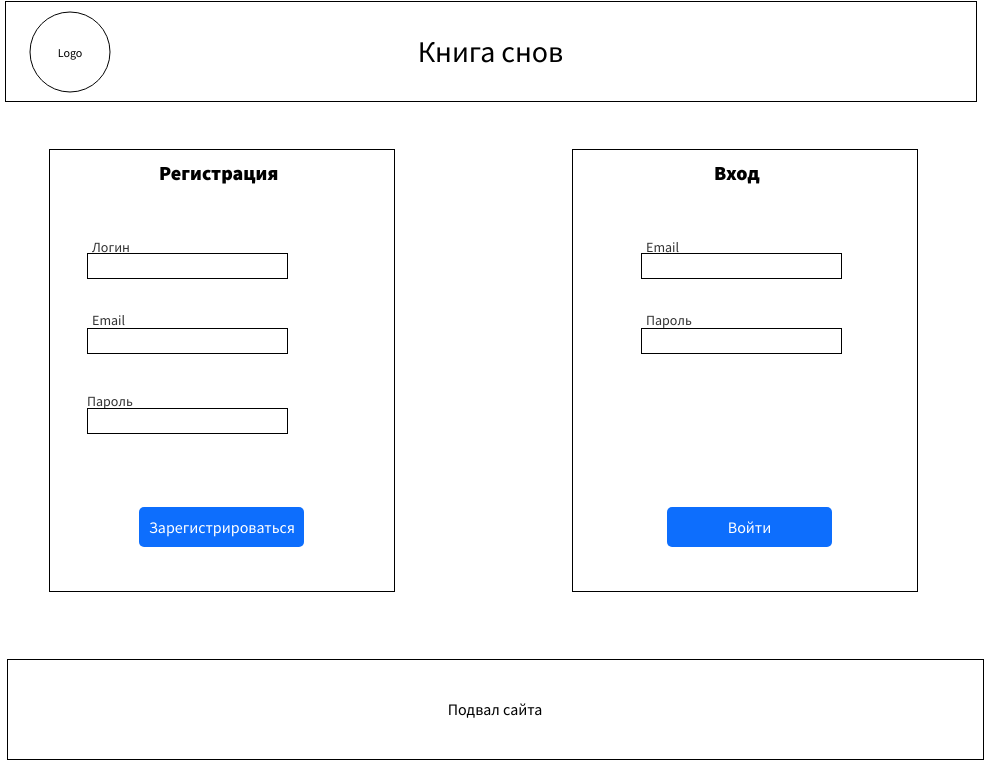
\includegraphics[width=0.65\textwidth]{img/1wf.png}
    \caption{Макет страницы входа и регистрации}
    \label{fig:mockup_login}
\end{figure}
\vspace{0.5cm}

\newpage
\textbf{Макет страницы «Моя книга снов».} 
На рисунке~\ref{fig:mockup_gallery} представлен макет личного кабинета пользователя. В верхней части расположена панель навигации с пунктами: «Моя книга», «Новый сон», «Статистика», «Профиль». Основная область содержит галерею карточек снов. Каждая карточка включает миниатюру изображения, заголовок, дату сна и оценку настроения. В правом верхнем углу находится кнопка «Новый сон» для быстрого создания записи.

\begin{figure}[ht!]
    \centering
    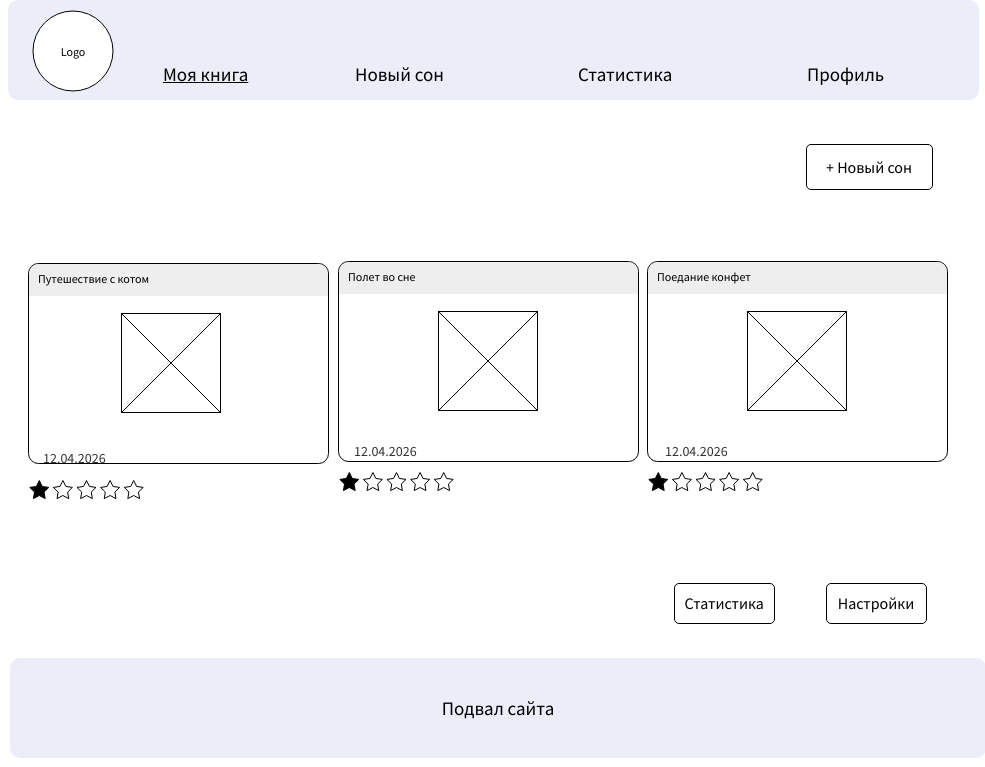
\includegraphics[width=0.65\textwidth]{img/2wf.png}
    \caption{Макет страницы «Моя книга снов»}
    \label{fig:mockup_gallery}
\end{figure}
\vspace{0.5cm}

\newpage
\textbf{Макет страницы создания и редактирования сна.} 
На рисунке~\ref{fig:mockup_create} представлен макет формы создания нового сна. Страница содержит следующие поля: заголовок, дата сна, оценка настроения, текст сна (многострочное поле). Внизу формы расположены кнопки «Сохранить» и «Отмена». Предусмотрена кнопка ИИ-генерации изображения, а также самостоятельного добавления картинки пользователем.

\begin{figure}[ht!]
    \centering
    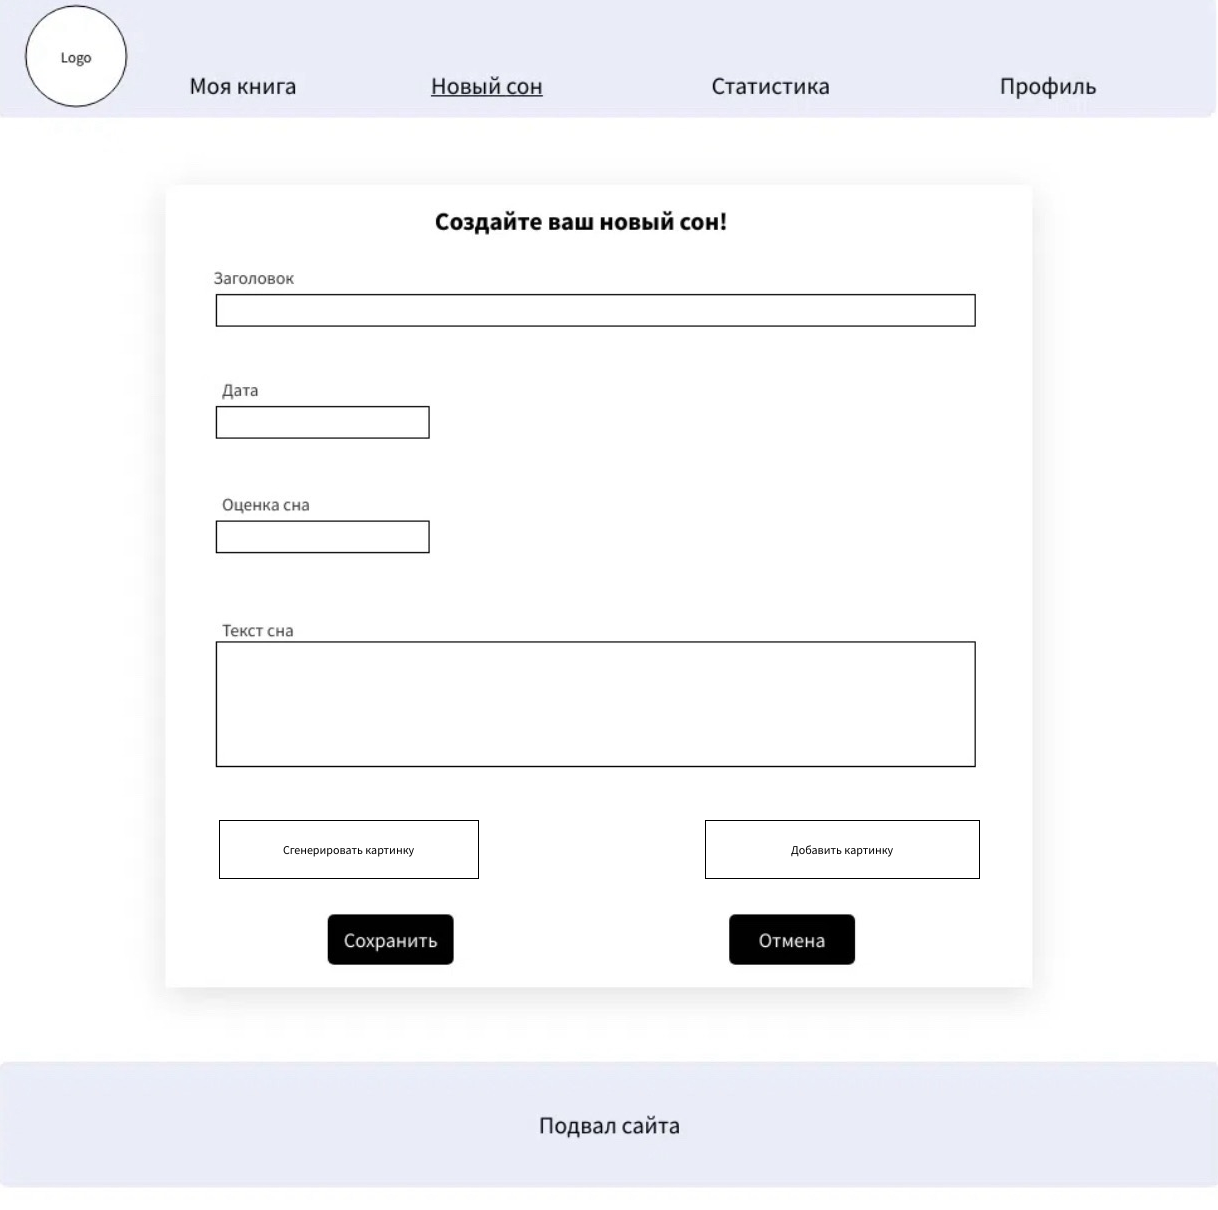
\includegraphics[width=0.65\textwidth]{img/3wf.png}
    \caption{Макет страницы создания и редактирования сна}
    \label{fig:mockup_create}
\end{figure}


\textbf{Макет страницы просмотра одного сна.} 
На рисунке~\ref{fig:mockup_detail} представлен макет детальной страницы сна. Страница разделена на две колонки: слева отображается изображение, справа — метаданные: дата сна, оценка настроения, список распознанных символов. Ниже располагается полный текст сна. Под текстом находятся кнопки «Редактировать», «Удалить» и «Перегенерировать картинку».

\begin{figure}[ht!]
    \centering
    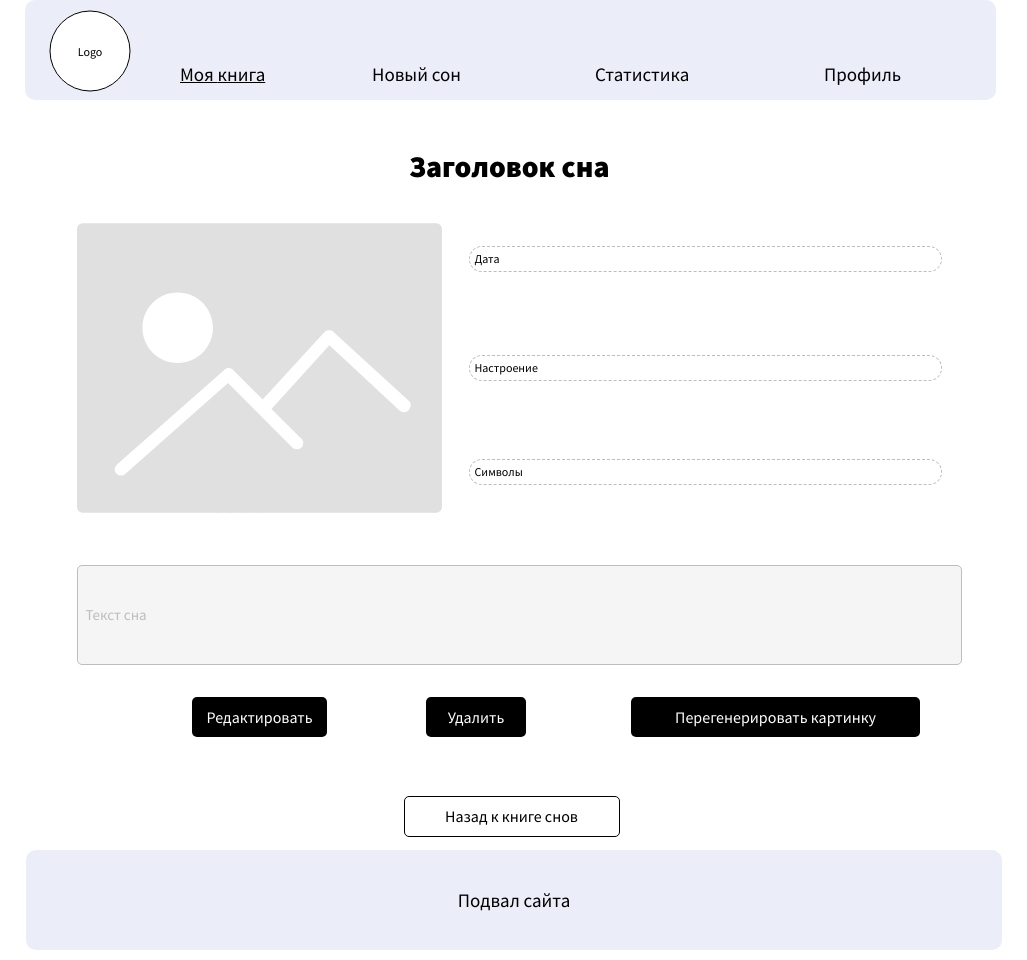
\includegraphics[width=0.65\textwidth]{img/4wf.png}
    \caption{Макет страницы просмотра одного сна}
    \label{fig:mockup_detail}
\end{figure}
\vspace{0.5cm}

\newpage
\textbf{Макет страницы статистики и аналитики.}

На рисунке~\ref{fig:mockup_stats} представлен макет страницы статистики. Страница содержит график эмоционального фона (линейный график изменения средней оценки настроения по датам), облако тегов (размер шрифта символа пропорционален частоте его встречаемости), блок «Топ-5 символов» и блок общей статистики (количество снов, средняя оценка, самый продуктивный месяц). В нижней части расположены кнопки экспорта статистики и всей книги снов в CSV.

\begin{figure}[ht!]
    \centering
    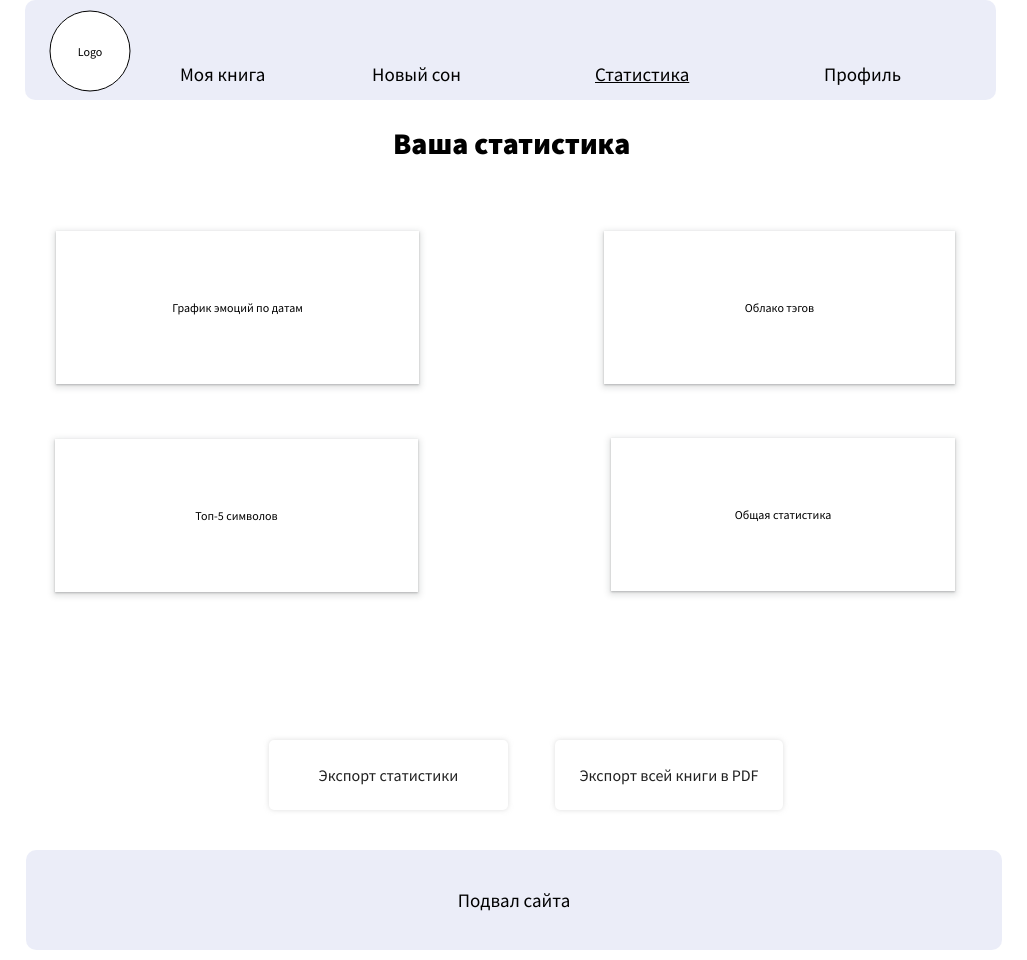
\includegraphics[width=0.65\textwidth]{img/5wf.png}
    \caption{Макет страницы статистики и аналитики}
    \label{fig:mockup_stats}
\end{figure}
\vspace{0.5cm}

\newpage
\textbf{Макет страницы профиля пользователя.}

На рисунке~\ref{fig:mockup_profile} представлен макет страницы профиля. В левой части отображается аватар пользователя, в правой — личные данные: имя пользователя, email, дата регистрации и роль. Ниже расположен блок краткой статистики (количество снов, средняя оценка настроения, самый частый символ). Внизу страницы расположены кнопка «Выйти из аккаунта».

\begin{figure}[ht!]
    \centering
    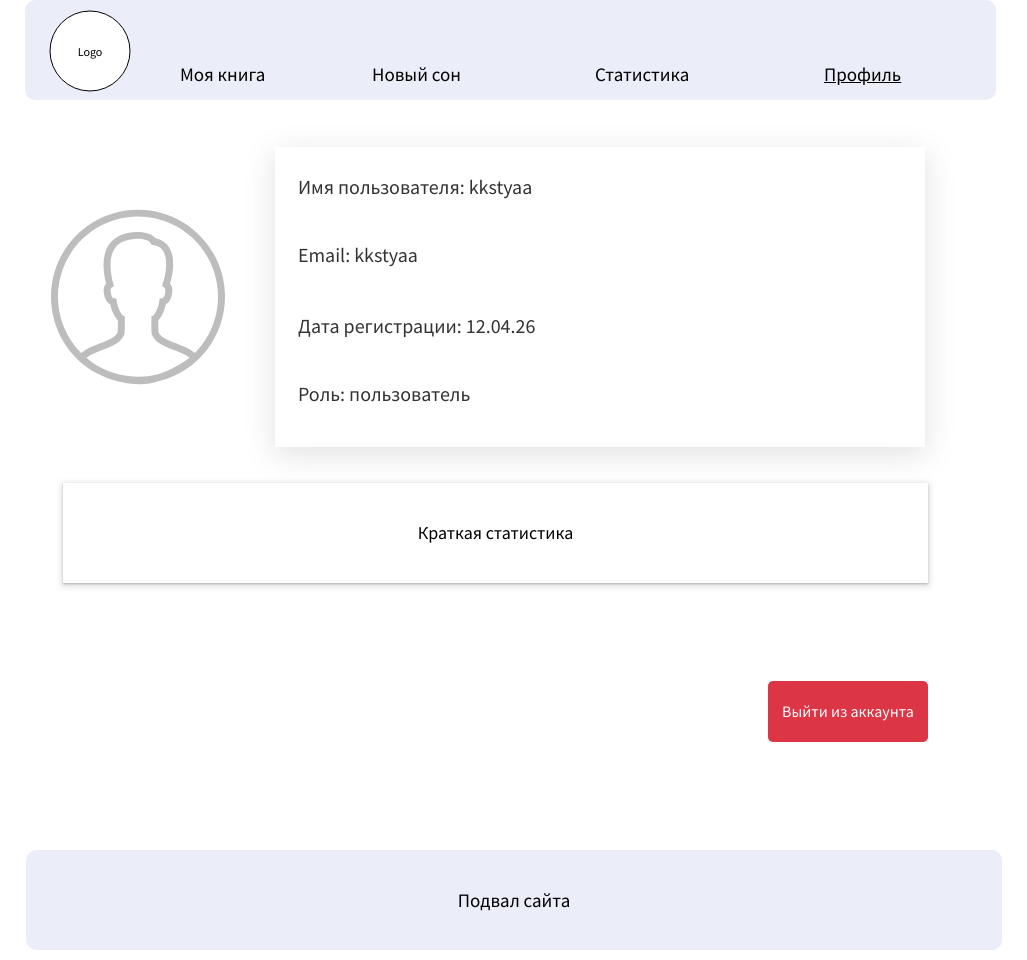
\includegraphics[width=0.65\textwidth]{img/6wf.png}
    \caption{Макет страницы профиля пользователя}
    \label{fig:mockup_profile}
\end{figure}
\vspace{0.5cm}
\newpage
Разработанные макеты охватывают весь ключевой функционал веб-приложения и служат основой для последующей программной реализации клиентской части.



% ==================== Глава 3 ====================
\newpage
\phantomsection
\section*{Глава 3. Разработка веб-приложения}
\addcontentsline{toc}{section}{Глава 3. Разработка веб-приложения}
\stepcounter{section}

\subsection{Модели базы данных}

В соответствии с задачей 3.1, была спроектирована объектно-реляционная модель базы данных с использованием библиотеки \textbf{Flask-SQLAlchemy}. Модели реализованы в виде Python-классов, отображаемых на таблицы реляционной базы данных SQLite. Пример модели пользователя представлен в листинге~\ref{lst:user_model}.

\begin{lstlisting}[caption={Модель пользователя}, label={lst:user_model}]
class User(db.Model, UserMixin):
    __tablename__ = 'users'

    user_id = db.Column(db.Integer, primary_key=True)
    username = db.Column(db.String(100), unique=True, nullable=False)
    email = db.Column(db.String(255), unique=True, nullable=False)
    password_hash = db.Column(db.String(255), nullable=False)
    role = db.Column(db.String(20), default='user')
    avatar_url = db.Column(db.String(500), nullable=True)
    created_at = db.Column(db.DateTime, default=datetime.now)

    dreams = db.relationship('Dream', backref='author', lazy=True)
    statistics = db.relationship('Statistic', backref='user', lazy=True)
    emotion_stats = db.relationship('EmotionStat', backref='user', lazy=True)
    symbol_stats = db.relationship('SymbolStat', backref='user', lazy=True)
    generation_requests = db.relationship('GenerationRequest', backref='user', lazy=True)
    user_images = db.relationship('UserImage', backref='user', lazy=True)

\end{lstlisting}

Листинг~\ref{lst:dream_model} демонстрирует модель сна, связанную с пользователем и символами.

\begin{lstlisting}[caption={Модель сна}, label={lst:dream_model}]
class Dream(db.Model):
    __tablename__ = 'dreams'

    dream_id = db.Column(db.Integer, primary_key=True)
    user_id = db.Column(db.Integer, db.ForeignKey('users.user_id'), nullable=False)
    title = db.Column(db.String(200), nullable=False)
    content = db.Column(db.Text, nullable=False)
    dream_date = db.Column(db.Date, nullable=False)
    mood = db.Column(db.Integer)
    created_at = db.Column(db.DateTime, default=datetime.now)
    updated_at = db.Column(db.DateTime, default=datetime.now, onupdate=datetime.now)

    # связи
    dream_symbols = db.relationship('DreamSymbol', backref='dream', lazy=True)
    generated_image = db.relationship('GeneratedImage', backref='dream', uselist=False)
    user_image = db.relationship('UserImage', backref='dream', uselist=False)
\end{lstlisting}

Всего в рамках проекта было реализовано 10 сущностей, что превышает минимальное требование (не менее 3).

\subsection{Аутентификация и личные кабинеты}

Согласно задаче 3.2, в системе реализована ролевая модель доступа с использованием библиотеки \textbf{Flask-Login}. Для обеспечения безопасности пароли пользователей хранятся в базе данных в хешированном виде (функция \texttt{generate\_password\_hash} из модуля \texttt{werkzeug.security}).

Листинг~\ref{lst:login} демонстрирует логику аутентификации пользователя.

\begin{lstlisting}[caption={Обработчик входа в систему}, label={lst:login}]
@bp.route('/login', methods=['GET', 'POST'])
def login():
    if current_user.is_authenticated:
        return redirect(url_for('index'))

    if request.method == 'POST':
        username = request.form.get('login')
        password = request.form.get('password')
        remember = request.form.get('remember')

        user = User.query.filter_by(username=username).first()

        if user and user.check_password(password):
            login_user(user, remember=bool(remember))
            flash('Вы успешно вошли в систему!', 'success')
            return redirect(url_for('index'))
        flash('Неверный логин или пароль', 'danger')

    return render_template('auth/login.html')
\end{lstlisting}

Для создания новой учётной записи реализован маршрут регистрации (листинг~\ref{lst:register}). Перед сохранением выполняется проверка уникальности логина и email, а также совпадения паролей.

\begin{lstlisting}[caption={Обработчик регистрации пользователя}, label={lst:register}]
@bp.route('/register', methods=['GET', 'POST'])
def register():
    if current_user.is_authenticated:
        return redirect(url_for('index'))

    if request.method == 'POST':
        username = request.form.get('login')
        email = request.form.get('email')
        password = request.form.get('password')
        confirm = request.form.get('confirm_password')

        if password != confirm:
            flash('Пароли не совпадают', 'danger')
            return redirect(url_for('auth.register'))

        if User.query.filter_by(username=username).first():
            flash('Пользователь с таким логином уже существует', 'danger')
            return redirect(url_for('auth.register'))

        if User.query.filter_by(email=email).first():
            flash('Пользователь с таким email уже существует', 'danger')
            return redirect(url_for('auth.register'))

        user = User(username=username, email=email)
        user.set_password(password)
        db.session.add(user)
        db.session.commit()

        login_user(user)
        flash('Регистрация прошла успешно!', 'success')
        return redirect(url_for('index'))

    return render_template('auth/register.html')
\end{lstlisting}

После успешной аутентификации пользователь перенаправляется в личный кабинет (страница профиля), где отображается его информация и краткая статистика. Пример шаблона страницы профиля представлен в листинге~\ref{lst:profile_template}.

\begin{lstlisting}[caption={Шаблон страницы профиля (profile.html)}, label={lst:profile_template}]
<div class="profile-container">
    <!-- Основная карточка профиля -->
    <div class="profile-card">
        <div class="row align-items-center">
            <!-- Аватар -->
            <div class="col-md-3 profile-avatar-section">
                <div class="avatar-circle">
                    {% if current_user.avatar_url %}
                        <img src="{{ current_user.avatar_url }}" class="avatar-img" alt="avatar" style="width: 100%; height: 100%; object-fit: cover; border-radius: 50%;">
                    {% else %}
                        <span class="avatar-text">{{ current_user.username[0]|upper }}</span>
                    {% endif %}
                </div>
                <form method="POST" action="{{ url_for('auth.upload_avatar') }}" enctype="multipart/form-data" class="mt-2">
                    <input type="file" name="avatar" accept="image/*" id="avatarInput" style="display: none;" onchange="this.form.submit()">
                    <label for="avatarInput" class="avatar-edit" style="cursor: pointer;">Сменить аватар</label>
                </form>
            </div>

            <!-- Информация о пользователе-->
            <div class="col-md-9 profile-info-section">
                <h1 class="profile-username">{{ current_user.username }}</h1>
                <span class="profile-role">{{ current_user.role|default('Пользователь') }}</span>

                <div class="profile-detail">
                    <span class="profile-detail-text">{{ current_user.email }}</span>
                </div>
                <div class="profile-detail">
                    <span class="profile-detail-text">Зарегистрирован: {{ current_user.created_at.strftime('%d.%m.%Y') }}</span>
                </div>
            </div>
        </div>
    </div>

\end{lstlisting}

Для выхода из системы используется маршрут \texttt{/logout}, который завершает сессию пользователя и перенаправляет на главную страницу. Ролевая модель доступа реализована через поле \texttt{role} в модели пользователя и декоратор \texttt{@admin\_required}, ограничивающий доступ к административным функциям.

\subsection{CRUD-интерфейс для управления снами}

В рамках задачи 3.3 реализован полноценный CRUD-интерфейс для управления записями снов. Все операции доступны только авторизованным пользователям и ограничены их собственными данными.


Листинг~\ref{lst:crud_create} иллюстрирует создание новой записи сна.

\begin{lstlisting}[caption={Создание сна}, label={lst:crud_create}]
@bp.route('/new', methods=['GET', 'POST'])
@login_required
def new():
    if request.method == 'POST':
        title = request.form.get('title')
        content = request.form.get('content')
        dream_date = datetime.strptime(
            request.form.get('dream_date'), '%Y-%m-%d'
        ).date()
        mood = request.form.get('mood', type=int)

        dream = Dream(
            user_id=current_user.user_id,
            title=title,
            content=content,
            dream_date=dream_date,
            mood=mood
        )
        db.session.add(dream)
        db.session.commit()
        flash('Сон успешно добавлен!', 'success')
        return redirect(url_for('dreams.index'))
    return render_template('dreams/form.html', dream=None)
\end{lstlisting}


Просмотр списка снов (листинг~\ref{lst:crud_index}) реализован с пагинацией — на одной странице отображается не более 9 записей.

\begin{lstlisting}[caption={Просмотр списка снов}, label={lst:crud_index}]
@bp.route('/')
@login_required
def index():
    page = request.args.get('page', 1, type=int)
    per_page = 9
    
    pagination = Dream.query.filter_by(
        user_id=current_user.user_id
    ).order_by(Dream.dream_date.desc()).paginate(
        page=page, per_page=per_page, error_out=False
    )
    dreams = pagination.items
    
    return render_template('dreams/index.html', 
                         dreams=dreams, pagination=pagination)
\end{lstlisting}

Просмотр детальной страницы одного сна (листинг~\ref{lst:crud_show}) выполняется по его идентификатору с проверкой прав доступа.

\begin{lstlisting}[caption={Просмотр одного сна}, label={lst:crud_show}]
@bp.route('/<int:dream_id>')
@login_required
def show(dream_id):
    dream = Dream.query.get_or_404(dream_id)
    if dream.user_id != current_user.user_id:
        flash('У вас нет доступа к этому сну', 'danger')
        return redirect(url_for('dreams.index'))
    return render_template('dreams/show.html', dream=dream)
\end{lstlisting}


Листинг~\ref{lst:crud_edit} демонстрирует редактирование существующей записи сна.

\begin{lstlisting}[caption={Редактирование сна}, label={lst:crud_edit}]
@bp.route('/<int:dream_id>/edit', methods=['GET', 'POST'])
@login_required
def edit(dream_id):
    dream = Dream.query.get_or_404(dream_id)
    if dream.user_id != current_user.user_id:
        flash('У вас нет доступа к этому сну', 'danger')
        return redirect(url_for('dreams.index'))

    if request.method == 'POST':
        dream.title = request.form.get('title')
        dream.content = request.form.get('content')
        dream.dream_date = datetime.strptime(
            request.form.get('dream_date'), '%Y-%m-%d'
        ).date()
        dream.mood = request.form.get('mood', type=int)
        dream.updated_at = datetime.now()
        db.session.commit()
        
        flash('Сон успешно обновлён!', 'success')
        return redirect(url_for('dreams.show', dream_id=dream.dream_id))

    return render_template('dreams/form.html', dream=dream)
\end{lstlisting}


Листинг~\ref{lst:crud_delete} показывает реализацию удаления записи сна.

\begin{lstlisting}[caption={Удаление сна}, label={lst:crud_delete}]
@bp.route('/<int:dream_id>/delete', methods=['GET', 'POST'])
@login_required
def delete(dream_id):
    """Удаление сна"""
    dream = Dream.query.get_or_404(dream_id)
    if dream.user_id != current_user.user_id:
        flash('У вас нет доступа к этому сну', 'danger')
        return redirect(url_for('dreams.index'))

    db.session.delete(dream)
    db.session.commit()
    update_all_stats(current_user.user_id)
    flash('Сон удалён', 'success')
    return redirect(url_for('dreams.index'))
\end{lstlisting}

Таким образом, реализованы все четыре базовые операции CRUD: создание, чтение (список и детальный просмотр), редактирование и удаление. Каждая операция сопровождается проверкой прав доступа (только владелец сна может его изменять или удалять) и всплывающими уведомлениями о результате выполнения.
\subsection{Загрузка файлов}

Согласно задаче 3.4, в приложении реализована функция загрузки файлов двух типов: аватар пользователя и иллюстрации к снам. Файлы сохраняются на сервер с генерацией уникального имени для предотвращения коллизий.
Для загрузки аватара используется отдельный маршрут \texttt{/auth/upload\_avatar} (листинг~\ref{lst:upload_avatar}). Форма загрузки расположена на странице профиля и отправляется автоматически после выбора файла.

\begin{lstlisting}[caption={Загрузка аватара пользователя}, label={lst:upload_avatar}]
@bp.route('/upload_avatar', methods=['POST'])
@login_required
def upload_avatar():
    if 'avatar' not in request.files:
        flash('Файл не выбран', 'danger')
        return redirect(url_for('profile'))

    file = request.files['avatar']
    filename = save_file(file, current_app.config['AVATAR_FOLDER'])

    if filename:
        current_user.avatar_url = f'/uploads/avatars/{filename}'
        db.session.commit()
        flash('Аватар успешно обновлён!', 'success')
    else:
        flash('Недопустимый формат файла', 'danger')

    return redirect(url_for('profile'))
\end{lstlisting}

Функция \texttt{save\_file} (листинг~\ref{lst:save_file}) является универсальной и используется как для аватаров, так и для иллюстраций к снам.

\begin{lstlisting}[caption={Универсальная функция сохранения файла}, label={lst:save_file}]
def save_file(file, folder):
    """Сохраняет файл и возвращает его имя"""
    if not file or file.filename == '':
        return None
    
    if not allowed_file(file.filename):
        return None
    
    # Генерируем уникальное имя файла
    ext = file.filename.rsplit('.', 1)[1].lower()
    filename = f"{uuid.uuid4().hex}.{ext}"
    
    filepath = os.path.join(folder, filename)
    file.save(filepath)
    
    return filename
\end{lstlisting}

Загрузка изображений к снам реализована непосредственно в форме создания и редактирования сна. При отправке формы файл обрабатывается и сохраняется в папку \texttt{uploads/dream\_images/}. Листинг~\ref{lst:upload_dream_image} демонстрирует фрагмент кода обработки загруженного изображения при создании сна.

\begin{lstlisting}[caption={Загрузка изображения к сну}, label={lst:upload_dream_image}]
if 'user_image' in request.files:
    file = request.files['user_image']
    if file and file.filename:
        filename = save_file(file, 
            current_app.config['DREAM_IMAGES_FOLDER'])
        if filename:
            user_image = UserImage(
                dream_id=dream.dream_id,
                user_id=current_user.user_id,
                image_url=f'/uploads/dream_images/{filename}'
            )
            db.session.add(user_image)
\end{lstlisting}

Для доступа к загруженным файлам реализован специальный маршрут (листинг~\ref{lst:serve_file}), который возвращает файл из директории \texttt{uploads}.

\begin{lstlisting}[caption={Маршрут для раздачи загруженных файлов}, label={lst:serve_file}]
@app.route('/uploads/<path:filename>')
    def uploaded_file(filename):
        return send_from_directory(app.config['UPLOAD_FOLDER'], filename)
\end{lstlisting}

В конфигурационном файле заданы ограничения на типы и размер загружаемых файлов (листинг~\ref{lst:upload_config}).

\begin{lstlisting}[caption={Настройки загрузки файлов в config.py}, label={lst:upload_config}]
UPLOAD_FOLDER = os.path.join(os.path.dirname(os.path.abspath(__file__)), 'uploads')
AVATAR_FOLDER = os.path.join(UPLOAD_FOLDER, 'avatars')
DREAM_IMAGES_FOLDER = os.path.join(UPLOAD_FOLDER, 'dream_images')
MAX_CONTENT_LENGTH = 16 * 1024 * 1024  # 16MB
ALLOWED_EXTENSIONS = {'png', 'jpg', 'jpeg', 'gif', 'webp'}
\end{lstlisting}

Таким образом, в приложении реализована полноценная загрузка файлов обоих типов с проверкой допустимых расширений, уникальной генерацией имён и корректной раздачей через статические маршруты.
\subsection{Анализ текста сна}

В соответствии с задачей 3.5, реализован модуль автоматического распознавания символов в тексте сна. Алгоритм ищет в тексте ключевые слова, соответствующие записям из справочника символов, и сохраняет связи в таблице \texttt{dream\_symbols}.

Листинг~\ref{lst:symbol_analyzer} показывает основную логику анализа.

\begin{lstlisting}[caption={Анализ текста и сохранение символов}, label={lst:symbol_analyzer}]
def analyze_and_save_symbols(dream_id, content):
    if not content:
        return
    
    # Получаем все символы из БД
    all_symbols = Symbol.query.all()
    
    if not all_symbols:
        return
    
    found_symbols = []
    content_lower = content.lower()
    
    for symbol in all_symbols:
        # Ищем слово целиком (не часть другого слова)
        pattern = r'\b' + re.escape(symbol.name.lower()) + r'\b'
        if re.search(pattern, content_lower):
            found_symbols.append(symbol)
    
    # Удаляем старые связи
    DreamSymbol.query.filter_by(dream_id=dream_id).delete()
    
    # Добавляем новые
    for symbol in found_symbols:
        dream_symbol = DreamSymbol(dream_id=dream_id, symbol_id=symbol.symbol_id)
        db.session.add(dream_symbol)
    
    db.session.commit()
\end{lstlisting}

Данная функция вызывается при создании и редактировании сна, обеспечивая актуальность связей между снами и символами.

\subsection{Агрегация данных и статистика}

Согласно задаче 3.6, в приложении реализован модуль агрегации данных для построения статистики. Расчёт выполняется на лету с использованием агрегатных функций SQLAlchemy, а также кэшируется в таблице \texttt{statistics} для ускорения отображения.

Листинг~\ref{lst:stats} демонстрирует расчёт количества снов и средней оценки.

\begin{lstlisting}[caption={Расчёт основных статистических показателей}, label={lst:stats}]
@bp.route('/')
@login_required
def index():
    user_id = current_user.user_id
    
    total_dreams = Dream.query.filter_by(user_id=user_id).count()
    avg_mood = db.session.query(
        func.avg(Dream.mood)
    ).filter_by(user_id=user_id).scalar()
    
    monthly_counts = db.session.query(
        func.strftime('%Y-%m', Dream.dream_date).label('month'),
        func.count(Dream.dream_id).label('count')
    ).filter_by(user_id=user_id).group_by('month').all()
    
    return render_template('statistics/index.html', 
                         total_dreams=total_dreams,
                         avg_mood=avg_mood,
                         monthly_counts=monthly_counts)
\end{lstlisting}

Для визуализации данных на фронтенде используется библиотека \textbf{Chart.js}, позволяющая строить столбчатые и линейные графики динамики снов и эмоционального фона.

\subsection{Экспорт в CSV}

В рамках задачи 3.7 реализован модуль экспорта данных в формат CSV. Пользователь может экспортировать как сводную статистику (общая статистика + топ-символы), так и полный список всех своих снов. Листинг~\ref{lst:export} демонстрирует экспорт книги снов.

\begin{lstlisting}[caption={Экспорт списка снов в CSV}, label={lst:export}]
@bp.route('/export/dreams')
@login_required
def export_dreams():
    """Экспорт всех снов (книги) в CSV"""
    user_id = current_user.user_id
    dreams = Dream.query.filter_by(user_id=user_id).order_by(Dream.dream_date.desc()).all()
    
    si = StringIO()
    cw = csv.writer(si, delimiter=';')
    cw.writerow(['ID', 'Заголовок', 'Дата сна', 'Настроение (1-5)', 'Текст сна', 'Дата создания'])
    
    for dream in dreams:
        cw.writerow([
            dream.dream_id,
            dream.title,
            dream.dream_date.strftime('%d.%m.%Y'),
            dream.mood or '',
            dream.content[:200] + '...' if len(dream.content) > 200 else dream.content,
            dream.created_at.strftime('%d.%m.%Y %H:%M')
        ])
    
    output = si.getvalue()
    try:
        output_bytes = output.encode('windows-1251')
    except:
        output_bytes = output.encode('utf-8-sig')
    
    return Response(
        output_bytes,
        mimetype='text/csv',
        headers={'Content-Disposition': 'attachment;filename=dreams_export.csv'}
    )
\end{lstlisting}

Экспорт статистики выполняется аналогично, но содержит агрегированные данные.

\subsection{Панель администратора}

Согласно задаче 3.8, реализована панель администратора с расширенными правами. Доступ к панели ограничен декоратором \texttt{@admin\_required}, который проверяет роль пользователя. Листинг~\ref{lst:admin} показывает пример управления символами.

\begin{lstlisting}[caption={Управление символами в админ-панели}, label={lst:admin}]
@bp.route('/symbols')
@login_required
@admin_required
def symbols():
    symbols_list = Symbol.query.order_by(Symbol.name).all()
    return render_template('admin/symbols.html', symbols=symbols_list)

@bp.route('/symbols/new', methods=['GET', 'POST'])
@login_required
@admin_required
def new_symbol():
    if request.method == 'POST':
        name = request.form.get('name', '').strip()
        if Symbol.query.filter_by(name=name).first():
            flash('Символ уже существует', 'danger')
            return redirect(url_for('admin.new_symbol'))
        
        symbol = Symbol(name=name)
        db.session.add(symbol)
        db.session.commit()
        flash('Символ добавлен', 'success')
        return redirect(url_for('admin.symbols'))
    return render_template('admin/symbol_form.html', symbol=None)
\end{lstlisting}

Администратор имеет возможность просматривать список всех пользователей, изменять их роли, удалять пользователей, а также добавлять, редактировать и удалять символы из справочника. Репозиторий проекта доступен по адресу: \url{https://github.com/kkstyaa/dream-book_project}
\newpage

% ==================== Глава 4 ====================

\section{Оформление итогов работы}

\subsection{Git-репозиторий}

В ходе выполнения курсового проекта велась работа с системой контроля версий \textbf{Git}. Все этапы разработки фиксировались в локальном репозитории, затем синхронизировались с удалённым хостингом \textbf{GitHub}. Это позволило отслеживать изменения кода, возвращаться к предыдущим версиям и обеспечивать резервное копирование проекта.

Репозиторий проекта доступен по адресу:
\begin{center}
    \url{https://github.com/kkstyaa/dream-book_project}
\end{center}

Структура репозитория включает:
\begin{itemize}
    \item папку \texttt{app/} — весь исходный код веб-приложения (модели, маршруты, шаблоны, статические файлы);
    \item файлы конфигурации (\texttt{config.py}, \texttt{requirements.txt});
    \item скрипт инициализации базы данных (\texttt{init\_db.py});
    \item точку входа в приложение (\texttt{run.py});
    \item документацию к проекту (папка \texttt{note/}).
\end{itemize}

\subsection{Деплой на хостинг}

Разработанное веб-приложение было развёрнуто на \textbf{PythonAnywhere} — хостинге, специализирующемся на размещении Python-приложений. Бесплатный тариф платформы предоставляет одно веб-приложение с возможностью использования базы данных SQLite, что полностью покрывает потребности проекта.

Процесс деплоя включал следующие шаги:
\begin{enumerate}
    \item Регистрация аккаунта на PythonAnywhere;
    \item Загрузка исходного кода проекта через веб-интерфейс;
    \item Установка зависимостей из \texttt{requirements.txt};
    \item Запуск скрипта инициализации базы данных \texttt{init\_db.py};
    \item Настройка статических маршрутов для CSS-файлов и загруженных пользователем изображений;
    \item Настройка WSGI-файла для корректного запуска Flask-приложения.
\end{enumerate}

После успешного деплоя приложение стало доступно по адресу:
\begin{center}
    \url{https://kkstyaa.pythonanywhere.com}
\end{center}

\subsection{Оформление отчёта}

Отчёт о курсовой работе оформлен в системе вёрстки Latex с использованием стилевого пакета \texttt{mospolytech\_coursework}, предоставленного университетом. Структура отчёта включает следующие разделы:

\begin{itemize}
    \item введение с обоснованием актуальности и постановкой задачи;
    \item анализ предметной области и обзор существующих решений;
    \item проектирование веб-приложения (анализ аудитории, функциональность, модель данных, макеты страниц);
    \item разработка веб-приложения с приведением листингов ключевых модулей;
    \item оформление итогов работы (Git-репозиторий, деплой на хостинг).
\end{itemize}

Все графические материалы (ER-диаграмма, Use Case-диаграмма, макеты страниц) выполнены с использованием инструментов \textbf{Draw.io} и \textbf{Mockflow}. Текст отчёта оформлен в соответствии с требованиями ГОСТ и методическими рекомендациями университета.

\newpage

% ==================== ЗАКЛЮЧЕНИЕ ====================

\section*{ЗАКЛЮЧЕНИЕ}
\addcontentsline{toc}{section}{ЗАКЛЮЧЕНИЕ}

В результате выполнения курсового проекта было разработано веб-приложение «Книга снов» — инструмент для ведения дневника сновидений с возможностью статистического анализа записей.

В ходе работы были решены все поставленные задачи:

\begin{enumerate}
    \item Проведён сравнительный анализ существующих решений для ведения дневников сновидений, выявлены их недостатки и обоснован выбор технологического стека (Flask, SQLite, Bootstrap 5).
    
    \item Разработана архитектура клиент-серверного приложения, спроектирована структура базы данных, состоящая из 10 таблиц, обеспечивающих хранение пользователей, снов, символов, статистики и данных об ИИ-генерации.
    
    \item Реализована система аутентификации и авторизации с использованием Flask-Login. Внедрена ролевая модель доступа (пользователь / администратор), администратор имеет доступ к панели управления пользователями и символами.
    
    \item Реализован полноценный CRUD-интерфейс для управления записями снов: создание, просмотр (с пагинацией), редактирование и удаление. Каждая операция защищена проверкой прав доступа.
    
    \item Разработан модуль агрегации данных для статистического анализа. Пользователю доступны график эмоционального фона, облако тегов, топ-5 символов, общая статистика, а также экспорт данных в CSV (как сводной статистики, так и полной книги снов).
    
    \item Выполнено оформление итогов работы: код размещён в публичном репозитории GitHub, приложение развёрнуто на хостинге PythonAnywhere.
\end{enumerate}

Приложение реализует заявленный функционал: пользователь может регистрироваться, создавать сны, добавлять к ним иллюстрации, просматривать статистику и экспортировать данные. Администратор управляет справочником символов и пользователями.

Таким образом, цель курсового проекта — проектирование и реализация клиент-серверного веб-приложения для ведения дневника сновидений — достигнута полностью.

\newpage

% ==================== СПИСОК ИСТОЧНИКОВ ====================

\section*{СПИСОК ИСПОЛЬЗОВАННЫХ ИСТОЧНИКОВ}
\addcontentsline{toc}{section}{СПИСОК ИСПОЛЬЗОВАННЫХ ИСТОЧНИКОВ}

\begin{enumerate}
    \item Курс СДО. Разработка веб-приложений [Электронный ресурс]. — Режим доступа: \url{https://lms.mospolytech.ru/course/view.php?id=16219} (дата обращения: 19.05.2026).
    
    \item Материалы по Latex [Электронный ресурс]. — Режим доступа: \url{https://lms.mospolytech.ru/pluginfile.php/1353734/mod_resource/content/1/latex3days.pdf} (дата обращения: 02.04.2026).

    \item Курс СДО. Разработка веб-приложений [Электронный ресурс]. — Режим доступа: \url{https://lms.mospolytech.ru/course/view.php?id=16219} (дата обращения: 19.05.2026).
    
    \item Dreamovy [Электронный ресурс]. — Режим доступа: \url{https://apps.apple.com/ru/app/dreamovy/id6751917234} (дата обращения: 05.04.2026).
    
    \item Awoken [Электронный ресурс]. — Режим доступа: \url{https://www.rustore.ru/catalog/app/com.lucid_dreaming.awoken} (дата обращения: 05.04.2026).
    
    \item Lucid Dreamer [Электронный ресурс]. — Режим доступа: \url{https://www.luciddreamer.com/} (дата обращения: 05.04.2026).
    
    \item PythonAnywhere Documentation [Электронный ресурс]. — Режим доступа: \url{https://help.pythonanywhere.com/} (дата обращения: 10.06.2026).
    
    \item Инструкция по деплою приложений на PythonAnywhere [Электронный ресурс]. — Режим доступа: \url{https://youtu.be/da9lYlksvOk} (дата обращения: 10.06.2026).
    
    \item Как создать портрет пользователя [Электронный ресурс]. — Режим доступа: \url{https://www.uplab.ru/blog/metod-person-kak-sozdat-portret-polzovatelya/} (дата обращения: 30.04.2026).
    
    \item User Story [Электронный ресурс]. — Режим доступа: \url{https://practicum.yandex.ru/blog/chto-takoe-user-story-i-kak-napisat/} (дата обращения: 06.06.2026).

    \item SQLAlchemy Documentation [Электронный ресурс]. — Режим доступа: \url{https://www.sqlalchemy.org/} (дата обращения: 05.06.2026).
    
    \item Bootstrap Documentation [Электронный ресурс]. — Режим доступа: \url{https://getbootstrap.com/} (дата обращения: 05.06.2026).
    
    \item Chart.js Documentation [Электронный ресурс]. — Режим доступа: \url{https://www.chartjs.org/} (дата обращения: 05.06.2026).
\end{enumerate}

\end{document}